\subsection{Contextual constraints}\label{subsec:contextualrestraints}
The grammar of Arc is a \gls{cfg} and only expresses the structure of the language. Further contextual constraints are required to specify if a program is well-formed and meaningfully correct. This section describes Arc's contextual constraints: the scope- and type rules.

\subsubsection{Scope rules}
The scope rules govern visibility, hiding some parts of a program from others. It also rules where certain things are allowed and others are not.

The Arduino language has static scope, with nested and flat block structures~\cite{cppref}. Blocks are declarable within other blocks (nested), but functions within other functions cannot(flat). Arc will have similar scope rules, making compilation more straightforward as source code and target code resemble each other regarding scope. Figure~\ref{fig:arcscoperules} shows a graphical model of Arc's scope rules.


\begin{figure}[htbp]
  \centering
  \missingfigure{Insert image of scope rules in Arc}
  \caption{Diagram of the scope structure of Arc.}
  \label{fig:arcscoperules}
\end{figure}


Arc statements and blocks, therefore, have nested scoping, while function declarations have a flat scope and are not declarable inside a scope. However, one key feature of Arc is its \textit{task} construct, which is not present in Arduino and requires particular focus.

A task declaration is like a function declaration and cannot be inside another scope. Additionally, declaring local variables inside the scope of a task declaration is not possible. The Protothreads implementation does not guarantee that the values of local variables are preserved when a thread becomes blocked, making it hard to know if using local variables in a thread will work as the programmer intended.

Another solution to this problem could be to hoist local variable declarations within a task declaration into the global scope. However, this could make static scopechecking more difficult. Listing~\ref{lst:hoistclash} shows how the hoisting of a locally declared variable may clash with globally declared variables. While the hoisting issue is not unsolvable, it is clearer to disallow variable declarations within a task declaration. Most importantly, writing an Arc task is entirely declarative - tasks are never called, unlike functions.


\begin{listing}[htb!]
  \begin{minted}[label=Scope clash]{text}
        num a = 1;
        task() {
            num a = 2; // hoist causes a clash here
        }
    \end{minted}
  \caption{Example of hoisting that causes a clash.}
  \label{lst:hoistclash}
\end{listing}


To describe the static scope rules of Arc with operational semantics, we use the environment-store model from Figure~\ref{fig:envstomodel}. The environment-store model describes variables as binding to locations, and locations binding to values, while the locations and values are then read with partial functions called \textit{environment} and \textit{store}.


\begin{figure}[htb!]
  \centering
  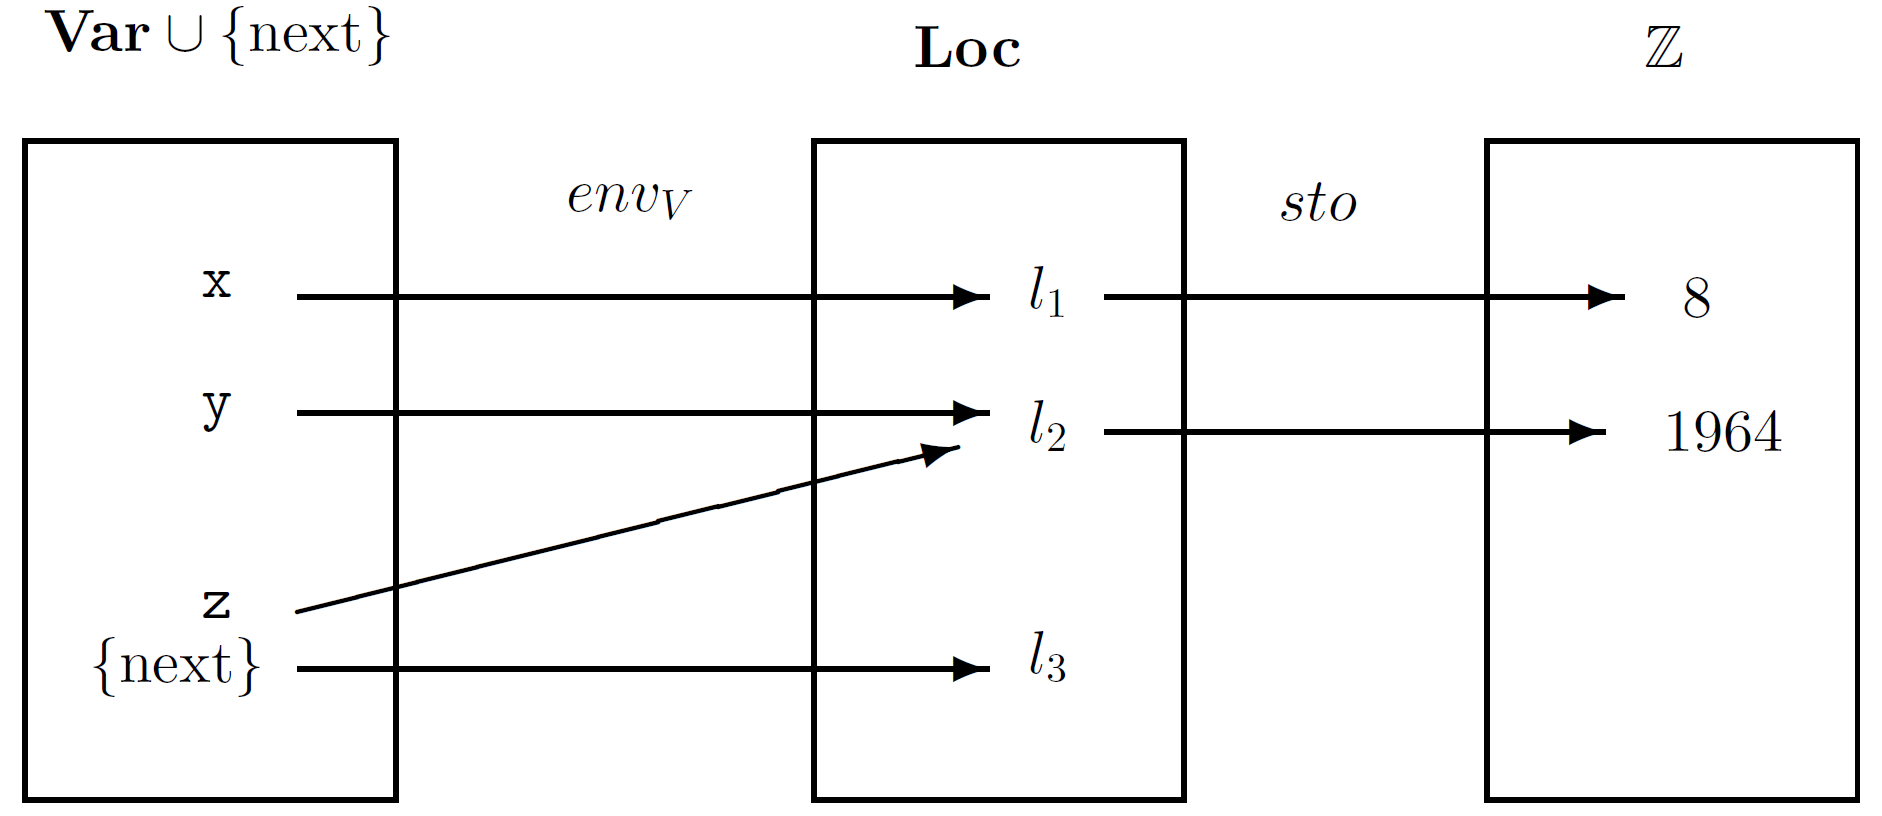
\includegraphics[width=0.8\textwidth]{figures/Environment_Store.png}
  \caption{Example diagram of the environment store model~\cite{Huttel2010}.}
  \label{fig:envstomodel}
\end{figure}


Arc has three environments: the variable environment, the function environment, and the task environment. To describe the semantics of these environments, some function, set and value names must be defined first. These definitions are presented in Table~\ref{tab:setsandfunctions}, and correspond to rules of Arc's \gls{cfg} described mathematically.

Following the standard of~\cite{Huttel2010}, sets are bolded and begins with a capital letter, while elements are not bolded.


\begin{table}[htb!]
  \centering
  \begin{tabular}{l}
    \toprule
    $\textbf{Val} = \textbf{Num} \cup \textbf{Bool} \cup \textbf{Char} \cup \textbf{Array} \cup \textbf{Pin}\ -$ Values                                                        \\
    $\textbf{Pin} = \textbf{PinValues} \times \textbf{Modes}\ -$ Pins are tuples of Arduino pins and modality                                                                  \\
    $\textbf{Array} = \mathbb{N} \rightharpoonup \textbf{Val} \setminus \textbf{Pin}\ -$ Arrays map numbers to non-pin values                                                  \\
    $\textbf{Par} = \textbf{Types} \times \textbf{Var}$                                                                                                                        \\
    $v \in \textbf{Val}\ -$ Literal values                                                                                                                                     \\
    $x \in \textbf{Var}\ -$ Variable id                                                                                                                                        \\
    $f \in \textbf{Fun}\ -$ Function id                                                                                                                                        \\
    $t \in \textbf{Types}\ -$ Type names                                                                                                                                       \\
    $y \in \mathcal{P} (\textbf{Par})\ -$ Formal parameter lists                                                                                                               \\
    $S \in \textbf{Stm}\ -$ Statements                                                                                                                                         \\
    $l \in \textbf{Loc}\ -$ An arbitrary location in \textbf{Loc}                                                                                                              \\
    next $\ -$ A special 'pointer' holding the value of the next element in \textbf{Loc}                                                                                       \\
    new $: \textbf{Loc} \rightarrow \textbf{Loc}\ -$ function to return succesor location                                                                                      \\
    \\
    $\textbf{Sto} = \textbf{Loc} \rightharpoonup \textbf{Val}\ -$ Set of stores                                                                                                \\
    $\textbf{Env}_V = \textbf{Var} \cup \{\text{next}\} \rightharpoonup \textbf{Loc}\ -$ Set of variable environments                                                          \\
    $\textbf{Env}_F = \textbf{Fun} \rightharpoonup \textbf{Stm} \times \mathcal{P} (\textbf{Par}) \times \textbf{Env}_V \times \textbf{Env}_F\ -$ Set of function environments \\
    $\textbf{Env}_T = \ -$ Set of task environments                                                                                                                            \\
    \bottomrule
  \end{tabular}
  \caption{Sets and function definitions.}
  \label{tab:setsandfunctions}
\end{table}

\supervisor{Should we define types as $\{ mut\} \times \textbf{Typenames} \cup \textbf{Typenames}$}


Additionally, we define the notation for updating a given environment $env_V \in \textbf{Env}_V$ we write $env_V[ x \mapsto l]$ to denote the update of $env_V$ given by


\begin{equation}
  env_V[x \mapsto l](y) =
  \begin{cases}
    env_V(y) & y \neq x \\
    l        & y = x
  \end{cases}
\end{equation}


and similarly for a $sto \in \textbf{Sto}$ we write $sto[ l \mapsto v ]$ to indicate the update of $sto$ given by


\begin{equation}
  sto[l \mapsto v](l^\prime) =
  \begin{cases}
    sto(l) & l \neq l^\prime \\
    v      & l = l^\prime
  \end{cases}
\end{equation}


With the above definitions of the environment store model and the scope rules, Arc's declarations can be described using operational semantics.


\begin{table}[htb!]
  \centering
  \begin{tabular}{ll}
    \toprule
    $[PIN_{DECL}]$  & $\dfrac
      {\langle env^{\prime\prime}_V, sto[l \mapsto v] \rangle \rightarrow (env^\prime_V, sto^\prime)}
      {\langle \text{'\#pin'} \ x = (pv, mode), env_V, sto\rangle\rightarrow (env^\prime_V, sto^\prime)}$ \\ [12pt]
                    & where $(pv, mode) \in \textbf{Pin} $                                                \\
                    & and $(pv,mode) \rightarrow v $                                                      \\
                    & and $l = env_V(\text{next})$                                                        \\
                    & and $env^{\prime\prime}_V = env_V[x \mapsto l][\text{next} \mapsto \text{new}(l)] $ \\
    \\

    $[VAR_{DECL}]$  & $\dfrac
      {\langle env^{\prime\prime}_V, sto[l \mapsto v] \rangle \rightarrow (env^\prime_V, sto^\prime)}
      {\langle t \ x = expr, env_V, sto\rangle\rightarrow (env^\prime_V, sto^\prime)}$                    \\ [12pt]
                    & where $env_V, sto \vdash expr \rightarrow v $                                       \\
                    & and $l = env_V(\text{next})$                                                        \\
                    & and $env^{\prime\prime}_V = env_V[x \mapsto l][\text{next} \mapsto \text{new}(l)] $ \\
    \\

    $[FUNC_{DECL}]$ & $\dfrac
      {env_V \vdash \langle env_F[f \mapsto \langle S, y, env_V, env_F\rangle] \rangle \rightarrow env^\prime_F}
      {env_V \vdash \langle t \ f (y) \{S \}, env_F \rangle \rightarrow env^\prime_F}$                    \\ [12pt]
    $[TASK_{DECL}]$ &                                                                                     \\
    \\


    \bottomrule
  \end{tabular}
  \caption{Arc's declarations and effects on scope defined with operational semantics.}
  \label{tab:arcscoperules}
\end{table}




\subsection{NOTES}:

Function call can't use recursion.
Function parameters are call by value.

Task parameters are mutable call by reference, and there can be only one mutable reference at a time.
Task semantics should contain the fact that the parameter list must not have multiple references to the same variable.

Can pin declarations and variable declarations be in the same environment?
What environment are tasks stored in, if any? Describe all 3 types.














